\documentclass[a4paper,12pt]{article}
\usepackage[a4paper, top = 1cm, bottom = 1.5cm, left = 1cm, right = 1cm, marginparwidth = 1cm]{geometry}

\usepackage{cmap}					% поиск в PDF
\usepackage[T2A]{fontenc}			% кодировка
\usepackage[utf8]{inputenc}			% кодировка исходного текста
\usepackage[english,russian]{babel}	% локализация и переносы

\usepackage{amsmath}
\usepackage{amssymb}
\usepackage{cancel}
\usepackage{graphicx}
\usepackage{float}
\usepackage{subfig}
\usepackage{tabularx}
\usepackage{longtable}
\usepackage[colorlinks=true, citecolor=red, linkcolor=red, urlcolor=blue]{hyperref}

\DeclareMathOperator\arctanh{arctanh}
\numberwithin{equation}{section}
\title{Первое задание}
\author{
	Хохлов Алексей \\
}

\begin{document}
	\maketitle
	
	Доделать: 1.3,1.4, 8 (возможно, доказывать необходимость)
	
	Везде, где будет необходимо доказать выпуклость множества или функции, будет
	подразумеваться, что $0 \leqslant \theta_i \leqslant 1$, $\sum \theta_i = 1$.
	Для доказательства афинности:$\sum \theta_i = 1$
	
	\section{Диаграмма Вороного}
	
	\subsection{}
	
	Условие $\Vert \mathbf{x} - \mathbf{x_0} \Vert_2 \leqslant \Vert \mathbf{x} -
	\mathbf{x_i} \Vert_2 , i=1,...,k$ означает, что
	
	\begin{equation}
	\sqrt {\sum_j (x_j-x_{0j})^2 }\leqslant \sqrt {\sum_j (x_j-x_{ij})^2 }
	\end{equation}
	
	Возведя в квадрат и перенеся в левую сторону, получим
	
	\begin{equation}
	\sum_j 2(x_{ij}-x_{0j})(x_j - \frac{x_{0j}+x_{ij}}{2}) \leqslant 0
	\end{equation}
	
	\begin{equation}
	\label{13}
	\sum_j 2(x_{ij}-x_{0j})x_j \leqslant  	\sum_j (x_{ij}-x_{0j}) (x_{0j}+x_{ij}) 
	\end{equation}
	
	Последнее неравенство можно представить в виде
	
	\begin{equation}
	\mathbf{A} \mathbf{x} \preceq \mathbf{b}
	\end{equation}
	где у матрицы $\mathbf{A}$ коэффициенты $ a_{ij} = 2(x_{ij}-x_{0j})$, а у
	столбца $ b_i = \sum\limits_{j} (x_{ij}-x_{0j}) (x_{0j}+x_{ij}) $
	
	Как видно, область Вороного является многоугольником.
	
	\subsection{}
	
	Попробуем из известных $\mathbf{A}$ и $\mathbf{b}$ восстановить точки.
	Выразим из $ (x_{ij}-x_{0j}) = a_{ij}/2$ точки $x_{ij}$
	
	\begin{equation}
	\label{15}
	x_{ij} = \frac{a_{ij}}{2} + x_{0j} 
	\end{equation}
	
	и подставим в $b_i$
	
	\begin{equation}
	b_i = \sum_j \frac{a_{ij}}{2}(\frac{a_{ij}}{2} + 2x_{0j}) = \frac14 \sum_j a_{ij}^2 + \sum_j a_{ij} x_{0j}
	\end{equation}
	
	\begin{equation}
	\label{17}
	\mathbf{A} \mathbf{x_0} = \mathbf{b} -  \frac 14  \mathbf{\tilde{a}}
	\end{equation}
	
	где столбец $\mathbf{\tilde{a}}$ таков, что их $i$ элементы --- сумма квадратов элементов $i$ строки матрицы $\mathbf{A}$ 
	
	Если матрица обратима, то
	
	\begin{equation}
	\mathbf{x_0} = \mathbf{A}^{-1} (\mathbf{b} - \frac 14  \mathbf{\tilde{a}})
	\end{equation}
	
	А из~\eqref{15} следует, что матрица $\mathbf{X}$, столбцы которой --- точки $\mathbf{x}_i$, такова:
	
	\begin{equation}
	\mathbf{X} = \frac 12 \mathbf{A} + \mathbf{A}^{-1} (\mathbf{b} - \frac 14  \mathbf{\tilde{a}})
	\end{equation}
	
	Если же матрица необратима, то в~\eqref{17} ищется пространство решений $\mathbf{x}_0$, и найденное решение подставляется в~\eqref{15}. Таким способом можно восстановить точки $\mathbf{x}_i$, $i=0,...,k$
	
	\subsection{}
	
	Заменим $\mathbf{x}_0$ на $\mathbf{x}_p$. Разбиение будет выглядеть следующим образом
	
	\subsection{}
	
	\section{Множество решений квадратного неравенства}
	
	\subsection{}
	
	Пусть $\mathbf{x_1}, \mathbf{x_2} \in C$ --- т.е. являются решениями
	неравенства. Узнаем, является ли $\mathbf{\tilde{x}} = \theta \mathbf{x_1} +
	(1-\theta)\mathbf{x_2}$ также решением. Пусть $f(\mathbf{x})$ --- квадратичная
	функция.
	
	\begin{equation}
	f(\mathbf{\tilde{x}}) = (\theta \mathbf{x_1^T} + (1-\theta)\mathbf{x_2^T})
	\mathbf{A} (\theta \mathbf{x_1} + (1-\theta)\mathbf{x_2})+ \mathbf{b^T} (\theta
	\mathbf{x_1} + (1-\theta)\mathbf{x_2}) + c
	\end{equation}
	
	Преобразуем квадратичное слагаемое 
	\begin{equation}
	\begin{split}
	& (\theta \mathbf{x_1^T} + (1-\theta)\mathbf{x_2^T}) \mathbf{A} (\theta
	\mathbf{x_1} + (1-\theta)\mathbf{x_2}) = \theta^2 \mathbf{x_1^T} \mathbf{A}
	\mathbf{x_1} +  (1-\theta)^2\mathbf{x_2^T}\mathbf{A}\mathbf{x_2} +
	\theta(1-\theta)\mathbf{x_1^T}\mathbf{A}\mathbf{x_2}+\theta(1-\theta)\mathbf{x_2^T}\mathbf{A}\mathbf{x_1}=
	\\
	&= \theta \mathbf{x_1^T} \mathbf{A} \mathbf{x_1} + 
	(1-\theta)\mathbf{x_2^T}\mathbf{A}\mathbf{x_2} - \theta (1 - \theta)
	\mathbf{x_1^T} \mathbf{A} \mathbf{x_1} - \theta
	(1-\theta)\mathbf{x_2^T}\mathbf{A}\mathbf{x_2} +
	\theta(1-\theta)\mathbf{x_1^T}\mathbf{A}\mathbf{x_2}+\theta(1-\theta)\mathbf{x_2^T}\mathbf{A}\mathbf{x_1}=\\
	&= \theta \mathbf{x_1^T} \mathbf{A} \mathbf{x_1} + 
	(1-\theta)\mathbf{x_2^T}\mathbf{A}\mathbf{x_2} + \theta(1-\theta)
	\left[\mathbf{x_1^T}\mathbf{A} (\mathbf{x_2} - \mathbf{x_1}) +
	\mathbf{x_2^T}\mathbf{A} (\mathbf{x_1} - \mathbf{x_2})\right] = \\
	&= \theta \mathbf{x_1^T} \mathbf{A} \mathbf{x_1} + 
	(1-\theta)\mathbf{x_2^T}\mathbf{A}\mathbf{x_2} - \theta(1-\theta)
	(\mathbf{x_2^T} - \mathbf{x_1^T})\mathbf{A} (\mathbf{x_2} - \mathbf{x_1}) 
	\end{split}
	\end{equation}
	
	Тогда квадратичная функция запишется в виде
	
	\begin{equation}
	\label{23}
	\begin{split}
	&f(\mathbf{\tilde{x}}) = \theta \mathbf{x_1^T} \mathbf{A} \mathbf{x_1} + \theta
	\mathbf{b^T}   \mathbf{x_1} +  \theta c +
	(1-\theta)\mathbf{x_2^T}\mathbf{A}\mathbf{x_2} + (1-\theta)\mathbf{b^T}
	\mathbf{x_2} + (1-\theta) c - \theta(1-\theta) (\mathbf{x_2^T} -
	\mathbf{x_1^T})\mathbf{A} (\mathbf{x_2} - \mathbf{x_1}) = \\
	&= \theta \left[ \mathbf{x_1^T} \mathbf{A} \mathbf{x_1} +  \mathbf{b^T}  
	\mathbf{x_1} + c \right] + (1-\theta) \left[ \mathbf{x_2^T} \mathbf{A}
	\mathbf{x_2} +  \mathbf{b^T}   \mathbf{x_2} + c \right]  - \theta(1-\theta)
	(\mathbf{x_2^T} - \mathbf{x_1^T})\mathbf{A} (\mathbf{x_2} - \mathbf{x_1}) 
	\end{split}
	\end{equation}
	Первое и второе слагаемое неположительны, т.к. удовлетворяют условию
	квадратичного неравенства. Если $\mathbf{A} \succ 0$, то 
	
	\begin{equation}
	-\theta(1-\theta) (\mathbf{x_2^T} - \mathbf{x_1^T})\mathbf{A} (\mathbf{x_2} -
	\mathbf{x_1}) =- \theta(1-\theta)
	\mathbf{\check{x}^T}\mathbf{A}\mathbf{\check{x}} \leqslant 0
	\end{equation}
	
	Итак, $\mathbf{\tilde{x}}$ также является решением, т.к.
	
	\begin{equation}
	f(\mathbf{\tilde{x}}) \leqslant 0
	\end{equation}
	
	Иными словами, множество решений квадратичного неравенства выпукло.
	
	\subsection{}
	
	Рассмотрим третье слагаемое в выражении~\eqref{23}
	
	\begin{equation}
	\label{26}
	\begin{split}
&	-\theta(1-\theta) (\mathbf{x_2^T} - \mathbf{x_1^T})\mathbf{A} (\mathbf{x_2} -
	\mathbf{x_1}) =\\
	&= -\theta(1-\theta) (\mathbf{x_2^T} - \mathbf{x_1^T})(\mathbf{A} + \lambda \mathbf{g}\mathbf{g}^\text{T}) (\mathbf{x_2} -
	\mathbf{x_1}) +\theta(1-\theta) (\mathbf{x_2^T} - \mathbf{x_1^T}) \lambda \mathbf{g}\mathbf{g}^\text{T} (\mathbf{x_2} -
	\mathbf{x_1})
	\end{split} 
	\end{equation}
	
	Первое слагаемое в~\eqref{26} неположительно, что следует из $\mathbf{A} + \lambda \mathbf{g}\mathbf{g}^\text{T} \succeq 0$. Изучим теперь второе слагаемое~\eqref{26}.
	
	Из определения гиперплоскости следует, что $\mathbf{g}^\text{T}\mathbf{x_1} = \mathbf{g}^\text{T}\mathbf{x_2}$, $\mathbf{x_1}^\text{T}\mathbf{g} = \mathbf{x_2}^\text{T}\mathbf{g}$.
	
	\begin{equation}
	\theta(1-\theta) (\mathbf{x_2^T} - \mathbf{x_1^T}) \lambda \mathbf{g}\mathbf{g}^\text{T} (\mathbf{x_2} -\mathbf{x_1}) = \theta(1-\theta)  ( \mathbf{x_2}^\text{T}\mathbf{g} - \mathbf{x_1}^\text{T}\mathbf{g}) (\mathbf{g}^\text{T} \mathbf{x_2} - \mathbf{g}^\text{T} \mathbf{x_1})=0
	\end{equation}
	
	Итак, для пересечения $C$ и гиперплоскости при условии $\mathbf{A} + \lambda \mathbf{g}\mathbf{g}^\text{T} \succeq 0$ выполнено 
	
	
	\begin{equation}
	\begin{split}
	&f(\mathbf{\tilde{x}}) \leqslant 0\\
	&\mathbf{g}^\text{T} \mathbf{\tilde{x}} + b =0
	\end{split}
	\end{equation}
	
	Значит, множество выпукло.
	
	\section{Выпуклый и аффинный}
	
	Для удобства будем обозначать в каждом пункте исследуемые множества буквой $C$.
	%1
	\subsection{}
	
	Проверим на выпуклость:
	\begin{equation}
	\alpha = \theta \alpha + (1 - \theta) \alpha \leqslant \mathbf{a^T} (\theta
	\mathbf{x_1} + (1 - \theta) \mathbf{x_2}) = \theta \mathbf{a^T} \mathbf{x_1} +
	(1 - \theta) \mathbf{a^T} \mathbf{x_2} \leqslant  \theta \beta + (1 - \theta)
	\beta = \beta 
	\end{equation}
	
	Множество выпукло. Проверим теперь на аффинность:
	
	Пусть $\alpha \neq \beta$, $\mathbf{a}^\text{T} \mathbf{x}_1 = \acute{\alpha}$, $\mathbf{a}^\text{T} \mathbf{x}_2 = \acute{\beta}$, $\alpha \leqslant \acute{\alpha} < \acute{\beta} \leqslant \beta$
	
	\begin{equation}
	\label{32}
	\mathbf{a^T} (\theta \mathbf{x_1} + (1 - \theta) \mathbf{x_2}) = \theta \acute{\alpha} + (1-\theta) \acute{\beta} =  \acute{\beta} + \theta (\acute{\alpha} - \acute{\beta})
	\end{equation}
	
	Если $\theta < 0$, то выражение~\eqref{32} больше, чем $\beta$, или, говоря иначе, $(\theta \mathbf{x_1} + (1 - \theta) \mathbf{x_2}) \notin C$. Множество не является аффинным.
	
	Если же $\alpha = \beta$, то множество будет удовлетворять уравнению прямой $\mathbf{a}^\text{T} \mathbf{x} = \alpha = \beta$. Такое множество будет аффинным:
	
	\begin{equation}
		\mathbf{a^T} (\theta \mathbf{x_1} + (1 - \theta) \mathbf{x_2}) = \theta \alpha + (1-\theta) \alpha = \alpha
	\end{equation}
	
	%2
	\subsection{}
	
	Проверим на выпуклость:
	\begin{equation}
	\mathbf{a_{1,2}^T} (\theta \mathbf{x_1} + (1 - \theta) \mathbf{x_2}) = \theta
	\mathbf{a_{1,2}^T} \mathbf{x_1} + (1 - \theta) \mathbf{a_{1,2}^T} \mathbf{x_2} \leqslant 
	\theta b_{1,2} + (1 - \theta) b_{1,2} = b_{1,2}
	\end{equation}
	
	Множество выпукло. Проверим теперь на аффинность:
	
	Пусть, во-первых, множество непусто, и вместе с тем $\mathbf{a_1^T} \neq -\mathbf{a_2^T}$, $b_1 \neq -b_2$.$\alpha = \mathbf{a_{1}^T} \mathbf{x_1}$, $\beta  = \mathbf{a_{1}^T} \mathbf{x_2}$,  $\alpha < \beta \leqslant b_1  $
	
	\begin{equation}
	\label{35}
	\mathbf{a_1^T} (\theta \mathbf{x_1} + (1 - \theta) \mathbf{x_2}) = \theta \alpha + (1-\theta) \beta= \beta + \theta(\alpha - \beta)
	\end{equation} 
	
		
	Пусть $\theta = \dfrac{b_1-\beta+1}{\alpha-\beta}$. Тогда
	
	\begin{equation}
	\beta + \theta(\alpha - \beta) = b_1 - 1 \geqslant b_1
	\end{equation}
	
	Множество не аффинно. 
	
	В случае же $\mathbf{a_1^T} = -\mathbf{a_2^T}$, $b_1 = -b_2$ Множество будет задавать прямую, а такое множество, как показано в пункте 1, аффинное.
	
	%3
	\subsection{}

	
	Проверим на выпуклость:
	
	Воспользуемся \eqref{13}, где $\mathbf{x}_i\in S$, а $\tilde{x_j} = \theta x_j^* + (1-\theta) x_j^{**}$. Неравенство
	
	\begin{equation}
	\theta\sum_j 2(x_{ij}-x_{0j}) x_j^* + (1-\theta) \sum_j 2(x_{ij}-x_{0j}) x_j^{**} \leqslant \sum_j (x_{ij}-x_{0j}) (x_{0j}+x_{ij}) 
	\end{equation}
	
	для любого $\mathbf{x}_i\in S$. Множество выпукло. Проверим теперь на аффинность:
	
	Пусть $\sum_j 2(x_{ij}-x_{0j}) x_j^* = b_i^*$, $\sum_j 2(x_{ij}-x_{0j}) x_j^{**} = b_i^{**}$, $b_i^* < b_i^{**} \leqslant b_i$, $\theta = \dfrac{b_i+1-b_i^*}{b_i^* - b_i^{**}}$
	
	\begin{equation}
	\theta\sum_j 2(x_{ij}-x_{0j}) x_j^* + (1-\theta) \sum_j 2(x_{ij}-x_{0j}) x_j^{**}  = b_i^{**} + \theta(b_i^* - b_i^{**}) = b_i +1 > b_i
	\end{equation}
	
	Множество не аффинно. В случае, если $S = \{\mathbf{x_0}\}$, то исследуемое множество --- $\mathbb{R}^n$, а такое множество аффинно.
	
	%4
	\subsection{}
	
	Условие $\Vert \mathbf{x} - \mathbf{a} \Vert_2 \leqslant \theta \Vert \mathbf{x} - \mathbf{b} \Vert_2$ равнозначно
	
	\begin{equation}
	\sum\limits_{i=1}^{n}\left[ (x_i - a_i)^2 - \theta^2 (x_i-b_i)^2 \right] = \sum\limits_{i=1}^{n}\left[(1-\theta^2)x_i^2 - 2(a_i-b_i)x_i + (a_i^2-b_i^2) \right] \leqslant 0
	\end{equation}
	
	Искомое множество --- множество решений квадратичного неравенства. Как было доказано в задаче 2, множество решений выпукло, если $\mathbf{A} \succ 0$. В нашем случае квадратичная форма такова: $\mathbf{A} = \text{diag}((1-\theta^2), ..., (1-\theta^2))$. Поскольку по условию $0 \leqslant \theta \leqslant 1$, то при $\theta < 1$ будет $(1-\theta^2) > 0$. Значит, все угловые миноры положительны, матрица положительно определена, и, следовательно, множество выпукло. При $\theta = 1$ множество будет $\Vert \mathbf{x} - \mathbf{a} \Vert_2 \leqslant  \Vert \mathbf{x} - \mathbf{b} \Vert_2$, которое, как было доказано, выпукло.
	
	Проверим теперь на аффинность:	
	
	Если $\theta = 1$, то, как показал пункт 3, множество не будет аффинным. Поскольку по условиям задачи $\theta \in \left[ 0;1 \right] $, то достаточно найти только одно такое $\theta$, что рушило бы аффинность множество. Однако если быть до конца честным, можно исследовать аффинность множества решений квадратичного неравенства, т.е. при $\theta \neq 1$. Пусть $\mathbf{x} = \alpha\mathbf{x}_1 + (1-\alpha)\mathbf{x}_2$, $\sum\limits_{i=1}^{n}\left[(1-\theta^2)x_{1i}^2 - 2(a_i-b_i)x_{1i} + (a_i^2-b_i^2) \right]  = y_1$, $\sum\limits_{i=1}^{n}\left[(1-\theta^2)x_{2i}^2 - 2(a_i-b_i)x_{2i} + (a_i^2-b_i^2) \right]  = y_2$, $y_2 > y_1$
	
	Легко видеть, что при 
	\begin{equation}
	\alpha < \frac12 \left(   \frac{y_1-y_2}{(1-\theta^2)\Vert \mathbf{x}_1 - \mathbf{x}_2 \Vert^2} - 1 \right)   \sqrt{\left( \frac{y_1-y_2}{(1-\theta^2)\Vert \mathbf{x}_1 - \mathbf{x}_2 \Vert^2} - 1\right)^2 -  \frac{4 y_2}{(1-\theta^2)\Vert \mathbf{x}_1 - \mathbf{x}_2 \Vert^2} }
	\end{equation}
	
	выполняется
	
	\begin{equation}
	\sum\limits_{i=1}^{n}\left[(1-\theta^2)\tilde{x}_i^2 - 2(a_i-b_i)\tilde{x}_i + (a_i^2-b_i^2) \right] > 0
	\end{equation}
	
	Множество не афинное.
	
	%5
	\subsection{}
	
	Проверим на выпуклость:
	
	\begin{equation}
	\mathbf{F_0} + \sum\limits_{i=1}^{n}(\theta x_{1i} + (1-\theta) x_{2i} )\mathbf{F_i} = \theta(\mathbf{F_0} + \sum\limits_{i=1}^{n} x_{1i}\mathbf{F_i}) + (1-\theta)(\mathbf{F_0} + \sum\limits_{i=1}^{n} x_{2i} \mathbf{F_i}) \succeq 0
	\end{equation}
	
	Множество выпукло. Проверим теперь на аффинность:
	
	Пусть  $\mathbf{a^T} \left[ \mathbf{F_0} + \sum\limits_{i=1}^{n} x_{1i} \mathbf{F_i}\right] \mathbf{a} = \alpha$, $\mathbf{a^T} \left[ \mathbf{F_0} + \sum\limits_{i=1}^{n} x_{2i} \mathbf{F_i}\right] \mathbf{a} = \beta$, $\beta > \alpha$
	
	\begin{equation}
	\mathbf{a^T} \left[ \mathbf{F_0} + \sum\limits_{i=1}^{n}(\theta x_{1i} + (1-\theta) x_{2i} )\mathbf{F_i} \right] \mathbf{a}= \beta + \theta (\alpha - \beta)
	\end{equation}
	
	При $\theta = \dfrac{-\beta - 1}{\alpha - \beta}$
	
	\begin{equation}
	\mathbf{a^T} \left[ \mathbf{F_0} + \sum\limits_{i=1}^{n}(\theta x_{1i} + (1-\theta) x_{2i} )\mathbf{F_i} \right] \mathbf{a} = -1 < 0
	\end{equation}
	
	Множество не аффинное.
	
	\section{Градиенты и гессианы}
	
	\subsection{}
	
	\subsubsection{a}
	
	Как известно, след матрицы --- сумма собственных чисел.
	
	\begin{equation}
	f(\mathbf{X}) = \text{Tr} (\mathbf{X}) = \sum_i x_{ii}
	\end{equation}
	
	Скалярное представление градиента:
	
	\begin{equation}
	\frac{\partial f(\mathbf{X}) }{\partial x_{pq}}  = \delta_{pq} 
	\end{equation}
	
	Векторное представление градиента:
	
	\begin{equation}
	\nabla f(\mathbf{X}) = \mathbf{I}
	\end{equation}
	
	\subsubsection{b}
	%TODO учесть нулевые собственные числа
	
	Из уравнения на собственные числа и теоремы Виета
	
	\begin{equation}
	\text{det}(\mathbf{X} - \lambda \mathbf{I}) = (-1)^n \lambda^n +(-1)^{n-1} \lambda^{n-1} \sum\limits_{i=1}^{n}x_{ii} + ... + \text{det} (\mathbf{X} - 0 \mathbf{I} )= 0
	\end{equation}
	
	следует, что 
	
	\begin{equation}
	\text{det} (\mathbf{X} )= \prod\limits_{i=1}^n \lambda_i  (\mathbf{X}) =
	f(\mathbf{X})
	\end{equation}
	Скалярное представление функции:
	
	\begin{equation}
	f(\mathbf{X}) = \sum_j (-1)^{i+j} x_{ij} M_{ij}
	\end{equation}
	
	Скалярное представление градиента:
	
	\begin{equation}
	\frac{\partial f(\mathbf{X}) }{\partial x_{pq}} = (-1)^{p+q}  M_{pq}
	\end{equation}
	
	Векторное представление градиента:
	
	\begin{equation}
	\nabla f(\mathbf{X})  = (\text{adj}(\mathbf{X}))^{\text{T}} =
	(\mathbf{X}^{-1}\cdot \text{det}(\mathbf{X}))^{\text{T}} =
	\text{det}(\mathbf{X}) \cdot\mathbf{X}^{\text{-T}}
	\end{equation}
	
	\subsection{}
	
	Матричное представление функции:
	
	\begin{equation}
	J(\mathbf{U}, \mathbf{V}) = \Vert \mathbf{U} \mathbf{V} - \mathbf{Y} \Vert_F^2
	+ \frac{\lambda}{2}(\Vert \mathbf{U} \Vert_F^2 + \Vert \mathbf{V}\Vert_F^2)
	\end{equation}
	
	Скалярное представление функции:
	
	\begin{equation}
	J(\mathbf{U}, \mathbf{V}) = \sum\limits_{i=1}^{n} \sum\limits_{j=1}^{n}
	(\sum\limits_{r=1}^{n}u_{ir}v_{rj}-y_{ij})^2 +
	\frac{\lambda}{2}\sum\limits_{i=1}^{n} \sum\limits_{j=1}^{n}(u_{ij}^2+v_{ij}^2)
	\end{equation}
	
	Скалярное представление градиентов:
	
	\begin{equation}
	\begin{split}
	&\frac{\partial J(\mathbf{U}, \mathbf{V})}{\partial u_{pq}} =
	\sum\limits_{j=1}^{n}2v_{qj} (\sum\limits_{r=1}^{n}u_{pr}v_{rj}-y_{pj}) +
	\lambda u_{pq} =\sum\limits_{j=1}^{n} \sum\limits_{r=1}^{n} 2v_{qj}
	u_{pr}v_{rj}-\sum\limits_{j=1}^{n} 2v_{qj} y_{pj} + \lambda u_{pq}= \\
	&=\sum\limits_{j=1}^{n} \sum\limits_{r=1}^{n} 2
	u_{pr}v_{rj}v_{jq}^\text{T}-\sum\limits_{j=1}^{n} 2 y_{pj}v_{jq}^\text{T} + \lambda u_{pq} = (2(\mathbf{U}\mathbf{V} -\mathbf{Y})\mathbf{V}^\text{T})_{pq} + \lambda (\mathbf{U})_{pq}
	\end{split}
	\end{equation}
	
	где $(\mathbf{A})_{pq}$ означает $pq$ компоненту $\mathbf{V}$. Аналогично и для
	градиента по $\mathbf{V}$
	\begin{equation}
	\begin{split}
	&\frac{\partial J(\mathbf{U}, \mathbf{V})}{\partial v_{pq}} =
	\sum\limits_{i=1}^{n}2u_{ip} (\sum\limits_{r=1}^{n}u_{ir}v_{rq}-y_{iq}) +
	\lambda v_{pq} = 2\sum\limits_{i=1}^{n} \sum\limits_{r=1}^{n} u_{pi}^\text{T}
	u_{ir}v_{rq}- 2\sum\limits_{i=1}^{n} u_{pi}^\text{T} y_{iq} + \lambda v_{pq} =
	\\
	&= 2 (\mathbf{U}^\text{T} (\mathbf{U}\mathbf{V} - \mathbf{Y}))_{pq} + \lambda
	(\mathbf{V})_{pq}  
	\end{split}
	\end{equation}
	
	Матричное представление градиентов:
	
	\begin{equation}
	\nabla_u J(\mathbf{U}, \mathbf{V}) = 2(\mathbf{U}\mathbf{V} -\mathbf{Y})\mathbf{V}^\text{T}  + \lambda \mathbf{U}
	\end{equation}
	
	
	\begin{equation}
	\nabla_v J(\mathbf{U}, \mathbf{V}) = 2 \mathbf{U}^\text{T} (\mathbf{U}\mathbf{V} - \mathbf{Y})+ \lambda \mathbf{V}
	\end{equation}
	
	\subsection{}
	
	Матричное представление функции:
	
	\begin{equation}
	f(\mathbf{w}) = \sum\limits_{i=1}^m \log (1+ e^{-y_i \mathbf{w^T x}_i})
	\end{equation}
	
	Скалярное представление:	
	\begin{equation}
	f(\mathbf{w}) = \sum\limits_{i=1}^m \log (1+ e^{-y_i \sum_j w_j x_{ij}})
	\end{equation}
	
	Скалярное представление градиента:
	
	\begin{equation}
	\frac{\partial f(\mathbf{w})}{\partial w_k} = \sum\limits_{i=1}^m  \frac{1}{1+
		e^{-y_i \mathbf{w^T x}_i}} \cdot e^{-y_i \mathbf{w^T x}_i} \cdot (-y_i x_{ik})
	\end{equation}
	
	Матричное представление градиента:
	
	%TODO раскрыть далее?
	\begin{equation}
	\nabla f(\mathbf{w}) = - \sum\limits_{i=1}^m  \frac{e^{-y_i \mathbf{w^T
				x}_i}}{1+ e^{-y_i \mathbf{w^T x}_i}} y_i\mathbf{x_i}
	\end{equation}
	
	Скалярное представление гессиана:
	\begin{equation}
	\frac{\partial^2 f(\mathbf{w})}{\partial w_k \partial w_p} =
	\sum\limits_{i=1}^m (-y_i x_{ik})  \frac{e^{-y_i \mathbf{w^T x}_i}\cdot(-y_i
		x_{ip})\cdot(1+e^{-y_i \mathbf{w^T x}_i})-e^{-y_i \mathbf{w^T x}_i}\cdot e^{-y_i
			\mathbf{w^T x}_i}\cdot(-y_i x_{ip})}{(1+e^{-y_i \mathbf{w^T x}_i})^2} 
	\end{equation}
	
	\begin{equation}
	\frac{\partial^2 f(\mathbf{w})}{\partial w_k \partial w_p}= \sum\limits_{i=1}^m
	y_i^2 x_{ik} x_{ip} \frac{e^{-y_i \mathbf{w^T x}_i}}{(1+e^{-y_i \mathbf{w^T
				x}_i})^2}
	\end{equation}	
	
	Матричное представление гессиана:
	\begin{equation}
	\mathbf{H} = \sum\limits_{i=1}^m y_i^2  \frac{e^{-y_i \mathbf{w^T
				x}_i}}{(1+e^{-y_i \mathbf{w^T x}_i})^2} \mathbf{x_i} \otimes
	\mathbf{x_i}^\text{T}
	\end{equation}
	
	\section{Кратчайший путь в графе}
	
	Пусть $\mathbf{c}$ --- вектор-столбец весов $(c_{pk}, c_{pq}, c_{qm},
	...)^{\text{T}}$ ориентированного взвешенного графа, и множество таких весов - выпуклое. Функция кратчайшего пути
	будет выглядеть следующим образом:
	
	\begin{equation}
	p_{ij}(\mathbf{c}) = \sum P_{pq}(\mathbf{c}) c_{pq}
	\end{equation}
	
	где 
	
	
	\begin{align}
	P_{pq}(\mathbf{c}) &=
	\left\{
	\begin{aligned}
	1 ,\; & (p,q) \subseteq (i,j) \\
	0 ,\; & (p,q) \nsubseteq (i,j)
	\end{aligned}
	\right. \\
	\end{align}
	
	или, иными словами, функция $P_{pq}(\mathbf{c})$ принимает значение 1, если
	ребро лежит в траектории с минимальным путём, и 0, если не лежит. Возьмем два
	произвольных столбца весов $\mathbf{c^a}$ и $\mathbf{c^b}$, а также столбец
	$\mathbf{\tilde{c}} = \theta \mathbf{c^a} + (1-\theta)\mathbf{c^b}$
	
	\begin{equation}
	p_{ij}(\mathbf{\tilde{c}}) = \sum P_{pq}(\mathbf{\tilde{c}}) (\theta c_{pq}^a +
	(1 - \theta) c_{pq}^b) = \theta \sum P_{pq}(\mathbf{\tilde{c}}) c_{pq}^a + (1 -
	\theta) \sum P_{pq}(\mathbf{\tilde{c}})  c_{pq}^b 
	\end{equation}
	
	Проверим на выпуклость или вогнутость:
	
	\begin{equation}
	\begin{split}
	&p_{ij}(\mathbf{\tilde{c}}) - \theta \sum P_{pq}(\mathbf{c^a}) c_{pq}^a - (1 -
	\theta) \sum P_{pq}(\mathbf{c^b})  c_{pq}^b \\
	&= \theta \left[ \sum P_{pq}(\mathbf{\tilde{c}}) c_{pq}^a - \sum
	P_{pq}(\mathbf{c^a}) c_{pq}^a \right]  + (1 - \theta) \left[ \sum
	P_{pq}(\mathbf{\tilde{c}}) c_{pq}^b - \sum P_{pq}(\mathbf{c^b}) c_{pq}^b\right] 
	\end{split}
	\end{equation}
	
	Поскольку $\sum P_{pq}(\mathbf{c^a}) c_{pq}^a$ и $\sum P_{pq}(\mathbf{c^b})
	c_{pq}^b$ --- кратчайшие пути для весов $\mathbf{c^a}$ и $\mathbf{c^b}$, то для
	любого иного вектора весов $\mathbf{\tilde{c}}$ выполнены неравенства
	
	\begin{equation}
	\begin{split}
	&\sum P_{pq}(\mathbf{\tilde{c}}) c_{pq}^a \geqslant \sum P_{pq}(\mathbf{c^a})
	c_{pq}^a \\
	&\sum P_{pq}(\mathbf{\tilde{c}}) c_{pq}^b \geqslant \sum P_{pq}(\mathbf{c^b})
	c_{pq}^b
	\end{split}
	\end{equation}	
	
	Следовательно, функция кратчайшего пути является вогнутой:
	
	\begin{equation}
	p_{ij}(\theta \mathbf{c^a} + (1 - \theta) \mathbf{c^b}) \geqslant \theta
	p_{ij}( \mathbf{c^a}) + (1-\theta ) p_{ij}( \mathbf{c^b}) 
	\end{equation}
	
	Эта вогнутость не является строгой. Рассмотрим граф
	
	\begin{figure}[H]
		\center{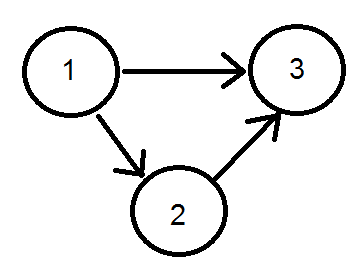
\includegraphics[width=0.4\textwidth]{./graph.png}}\\
		\caption{Граф.}
	\end{figure}
	
	Пусть $c_{13}^a = 2, c_{13}^b = 6, c_{12}^a = 1, c_{12}^b = 1, c_{23}^a = 2,
	c_{23}^b = 2$. Тогда $p_{13}(\mathbf{c^a}) = 2, p_{13}(\mathbf{c^b}) = 4$. Пусть
	$\theta = 0.5$. Для $\mathbf{\tilde{c}}$ веса будут $c_{13} = 4, c_{12} = 1.5,
	c_{23} = 1.5$, а минимальный путь $p_{13}(\mathbf{\tilde{c}}) = 3$. Отсюда
	$p_{13}(\mathbf{\tilde{c}}) = 0.5 p_{13}(\mathbf{c^a}) + 0.5
	p_{13}(\mathbf{c^b}) $. Как видим, строгого неравенства не наблюдается, и
	функция кратчайшего пути оказывается нестрого вогнутой.
	
	\section{Логарифмический барьер для конуса второго порядка}
	
	Итак, как обычно, пусть $\mathbf{\tilde{x}} = \theta \mathbf{x_1} +  (1 -
	\theta) \mathbf{x_2}$, $\tilde{t} = \theta t_1 + (1 - \theta) t_2$
	
	Раскроем аргумент логарифма:
	
	\begin{equation}
	\begin{split}
	&\tilde{t}^2 - \mathbf{\tilde{x}}^\text{T} \mathbf{\tilde{x}} = \theta^2 t_1^2
	+ (1-\theta)^2 t_2^2 + 2\theta(1-\theta)t_1 t_2 - \theta^2 \mathbf{x}_1^{T} -(1-
	\theta)^2 \mathbf{x}_2^{T} - \theta (1- \theta)\mathbf{x_1}^\text{T}
	\mathbf{x_2} - \theta (1- \theta)\mathbf{x_2}^\text{T} \mathbf{x_1} = \\
	&=\theta^2(t_1^2 - \mathbf{x_1}^\text{T} \mathbf{x_1}) + (1-\theta)^2(t_2^2 -
	\mathbf{x_2}^\text{T} \mathbf{x_2}) - 2\theta (1-\theta)(t_1 t_2 -
	\mathbf{x_1}^\text{T} \mathbf{x_2})
	\end{split}
	\end{equation}
	
	Проверим, верно ли неравенство
	
	\begin{equation}
	\label{62}
	\tilde{t}^2 - \mathbf{\tilde{x}}^\text{T} \mathbf{\tilde{x}} \geqslant \theta
	(t_1^2 - \mathbf{x_1}^\text{T} \mathbf{x_1}) + (1-\theta)(t_2^2 -
	\mathbf{x_2}^\text{T} \mathbf{x_2})
	\end{equation}
	
	Вычтем правую часть из левого и получим
	
	
	
	\begin{equation}
	\begin{split}
	\label{63}
	&\tilde{t}^2 - \mathbf{\tilde{x}}^\text{T} \mathbf{\tilde{x}} - \theta (t_1^2 -
	\mathbf{x_1}^\text{T} \mathbf{x_1}) + (1-\theta)(t_2^2 - \mathbf{x_2}^\text{T}
	\mathbf{x_2}) = \\
	&= \theta(1-\theta) \left[ (t_1^2 - \mathbf{x_1}^\text{T} \mathbf{x_1}) +
	(t_2^2 - \mathbf{x_2}^\text{T} \mathbf{x_2}) - 2(t_1 t_2 - \mathbf{x_1}^\text{T}
	\mathbf{x_2})\right] = \\
	&=\theta(1-\theta) \left[ (t_1-t_2)^2 - (\mathbf{x_2} -
	\mathbf{x_1})^\text{T}(\mathbf{x_2} - \mathbf{x_1})\right] 
	\end{split}
	\end{equation}
	
	%TODO ||x|| < t
	Множество $E$ таково, что $\Vert x \Vert_2 < t$. Следовательно,
	выражение~\eqref{63} больше нуля, а значит, неравенство~\eqref{62} верно. Плюс ко всему, множество $E$, очевидно, выпукло.
	
	Теперь проверим неравенство
	
	\begin{equation}
	\label{64}
	-\log(\tilde{t}^2 - \mathbf{\tilde{x}}^\text{T} \mathbf{\tilde{x}}) \leqslant -
	\theta \log(t_1^2 - \mathbf{x_1}^\text{T} \mathbf{x_1}) - (1-\theta) \log(t_2^2
	- \mathbf{x_2}^\text{T} \mathbf{x_2})
	\end{equation}
	
	Избавляясь от логарифмов, получим
	
	\begin{equation}
	\label{65}
	(\tilde{t}^2 - \mathbf{\tilde{x}}^\text{T} \mathbf{\tilde{x}}) \geqslant (t_1^2
	- \mathbf{x_1}^\text{T} \mathbf{x_1})^{\theta} (t_2^2 - \mathbf{x_2}^\text{T}
	\mathbf{x_2})^{1-\theta}
	\end{equation}
	
	Воспользуемся неравенством Юнга
	
	\begin{equation}
	a^\theta b^{1-\theta} \leqslant \theta a + (1-\theta) b
	\end{equation}
	
	Из неравенства Юнга и~\eqref{62} следует
	
	\begin{equation}
	(\tilde{t}^2 - \mathbf{\tilde{x}}^\text{T} \mathbf{\tilde{x}})\geqslant \theta
	(t_1^2 - \mathbf{x_1}^\text{T} \mathbf{x_1}) + (1-\theta)(t_2^2 -
	\mathbf{x_2}^\text{T} \mathbf{x_2}) \geqslant (t_1^2 - \mathbf{x_1}^\text{T}
	\mathbf{x_1})^{\theta} (t_2^2 - \mathbf{x_2}^\text{T} \mathbf{x_2})^{1-\theta}
	\end{equation}
	
	Отсюда следует, что неравенство~\eqref{65} верно, и вместе с ним верно
	~\eqref{64}. И, следовательно, логарифмический барьер для конуса второго порядка
	является выпуклым на множестве $E$.
	
	\section{Обратное неравенство Йенсена}
	
	Необходимо доказать, что
	
	\begin{equation}
	f(\lambda_1 \mathbf{x_1} + ... + \lambda_n \mathbf{x_n} ) \geqslant \lambda_1
	f(\mathbf{x_1}) + ... + \lambda_n f(\mathbf{x_n})
	\end{equation}
	
	Докажем неравенство, равносильное данному
	
	\begin{equation}
	f(\mathbf{x_1})  \leqslant \frac{1}{\lambda_1}f(\lambda_1 \mathbf{x_1} +
	...+\lambda_n\mathbf{x_n})  + \sum\limits_{i=2}^{n}
	(-\frac{\lambda_i}{\lambda_1} )  f(\mathbf{x_i})
	\end{equation}
	
	Сделаем преобразование переменных. Пусть $\sum\limits_{i=1}^{n} \lambda_i
	\mathbf{x_i} = \mathbf{\tilde{x_1}}$, $\mathbf{x_i} = \mathbf{\tilde{x_i}},
	i=2,...,n$. Неравенство преобразуется в
	
	\begin{equation}
	f(\frac{1}{\lambda_1}\mathbf{\tilde{x_1}}  + \sum\limits_{i=2}^{n}
	(-\frac{\lambda_i}{\lambda_1} )  \mathbf{\tilde{x_i}})  \leqslant
	\frac{1}{\lambda_1}f(\mathbf{\tilde{x_1}})  + \sum\limits_{i=2}^{n}
	(-\frac{\lambda_i}{\lambda_1} )  f(\mathbf{\tilde{x_i}})
	\end{equation}
	
	Поскольку $\lambda_1 > 0$, $\lambda_i \leqslant 0, i=2,...,n$, то $\lambda_1 =
	1 - \sum\limits_{i=2}^{n}\lambda_i \geqslant 1$, и, соответственно, $0 <
	\dfrac{1}{\lambda_1} \leqslant 1$. 
	
	В то же время $\lambda_1 = 1 - \sum\limits_{i=2}^{n}\lambda_i = 1 +
	\sum\limits_{i=2}^{n}(-\lambda_i) = 1 + \sum\limits_{i=2}^{n}\left|
	\lambda_i\right| > \left| \lambda_i\right|$, и, следовательно, $0 \leqslant
	(-\dfrac{\lambda_i}{\lambda_1}) < 1$.
	
	Переобозначим $\theta_1 = \dfrac{1}{\lambda_1}$, $\theta_i =
	(-\dfrac{\lambda_i}{\lambda_1}), i=2,...,n$. 
	
	Как видно, $0<\theta_1 \leqslant 1$, $0 \leqslant \theta_i < 1$, $\sum\limits_i
	\theta_i = \dfrac{1 - \sum\limits_{i=2}^{n}\lambda_i}{\lambda_1}=1$. Неравенство
	перепишется в виде
	
	\begin{equation}
	f( \sum\limits_{i=1}^{n} \theta_i \mathbf{\tilde{x_i}})  \leqslant
	\sum\limits_{i=1}^{n} \theta_i  f(\mathbf{\tilde{x_i}})
	\end{equation}
	
	Поскольку функция выпукла, то неравенство верно (неравенство Йенсена).
	
	\section{Выпуклая композиция}
	
	Пусть функция $\mathbf{y} = f(\mathbf{x})$ определена на множестве
	$\mathbf{X}$, а $h(\mathbf{y})$ на множестве $\mathbf{Y} = f(\mathbf{X})$. Их суперпозиция $g(\mathbf{x}) = h(f(\mathbf{x}))$. Также
	будем придерживаться следующих обозначений:
	\begin{equation}
	\begin{split}
	 &\mathbf{\tilde{x}} = \theta
	\mathbf{x_1} + (1-\theta )\mathbf{x_1}\\
	&\tilde{y} = f(\theta \mathbf{x_1} +
	(1-\theta )\mathbf{x_2})\\
	 &\tilde{\tilde{y}} = \theta  f(\mathbf{x_1})
	+ (1-\theta )f(\mathbf{x_2}) =\theta  y_1 + (1-\theta )y_2  . 
	\end{split}
	\end{equation}
	
	Рассмотрим следующие случаи:
	
	\subsection{$f(\mathbf{x})$ --- выпуклая, $h(y)$ --- выпуклая и нестрого
		возрастающая}
	
	Т.к. $f(\mathbf{x})$ --- выпуклая, то $\tilde{y} \leqslant \tilde{\tilde{y}}$.
	Поскольку $h(y)$ --- нестрого возрастающая, то $ h(\tilde{y}) \leqslant
	h({\tilde{\tilde{y}}})$. А из выпуклости $h(y)$ следует, что
	$h(\tilde{\tilde{y}}) \leqslant \theta h(y_1) + (1 - \theta) h(y_2)$
	
	\begin{equation}
	h(f(\mathbf{\tilde{x}})) =h( \tilde{y}) \leqslant h(\tilde{\tilde{y}})
	\leqslant \theta h(y_1) + (1 - \theta) h(y_2) = \theta h(f(\mathbf{x_1})) + (1 -
	\theta) h(f(\mathbf{x_2}))
	\end{equation}
	
	Выпуклость $f$, выпуклость и неубывающая монотонность $h$ одновременно ---
	достаточное условие для выпуклости суперпозиции.
	
	\subsection{$f(\mathbf{x})$ --- вогнутая, $h(y)$ --- выпуклая и нестрого
		убывающая}
	
	Из вогнутости $f(\mathbf{x})$ следует $\tilde{y} \geqslant \tilde{\tilde{y}}$.
	Из невозрастания $h(y)$ следует $ h(\tilde{y}) \leqslant
	h({\tilde{\tilde{y}}})$. А из выпуклости $h(y)$ следует, что
	$h(\tilde{\tilde{y}}) \leqslant \theta h(y_1) + (1 - \theta) h(y_2)$
	
	\begin{equation}
	h(f(\mathbf{\tilde{x}})) =h( \tilde{y}) \leqslant h(\tilde{\tilde{y}})
	\leqslant \theta h(y_1) + (1 - \theta) h(y_2) = \theta h(f(\mathbf{x_1})) + (1 -
	\theta) h(f(\mathbf{x_2}))
	\end{equation}
	
	Вогнутость $f$, выпуклость и невозрастающая монотонность $h$ одновременно ---
	достаточное условие для выпуклости суперпозиции.
	
	\subsection{$f(\mathbf{x})$ и $h(y)$ --- дважды дифференциируемы}
	
	\begin{equation}
	\frac{\partial g}{\partial x_i} = h^{\prime} \frac{\partial f}{\partial x_i}
	\end{equation}
	
	\begin{equation}
	\frac{\partial^2 g}{\partial x_i \partial x_j} = h^{\prime\prime} \frac{\partial f}{\partial x_i}\frac{\partial f}{\partial x_j} + h^{\prime} \frac{\partial^2 f}{\partial x_i\partial x_j}
	\end{equation}
	
	\begin{equation}
	\mathbf{H_g} = h^{\prime\prime} \nabla f \otimes (\nabla f)^\text{T} + h^{\prime} \mathbf{H_f}
	\end{equation}
	
	Гессиан представляет собой матрицу вида
	
	$\mathbf{H_g} =\left( \begin{matrix}
		h^{\prime\prime} \left( \dfrac{\partial f}{\partial x_i}\right)^2 + h^{\prime} \dfrac{\partial^2 f}{\partial x_i^2} & ... & h^{\prime\prime}  \dfrac{\partial f}{\partial x_i}\dfrac{\partial f}{\partial x_j} + h^{\prime} \dfrac{\partial^2 f}{\partial x_i \partial x_j} \\
		... & ... & ... \\
		h^{\prime\prime}  \dfrac{\partial f}{\partial x_j}\dfrac{\partial f}{\partial x_i} + h^{\prime} \dfrac{\partial^2 f}{\partial x_j \partial x_i} & ... & h^{\prime\prime} \left( \dfrac{\partial f}{\partial x_j}\right)^2 + h^{\prime} \dfrac{\partial^2 f}{\partial x_j^2} \\
	\end{matrix}\right) $
	
	%TODO необходимое и достаточное условие
	
	Для положительной полуопределенности необходимо и достаточно, чтобы угловые миноры были неотрицательны. Как минимум, необходимо, чтобы для любого $j$ выполнялось условие
	
	\begin{equation}
	h^{\prime\prime} \left( \dfrac{\partial f}{\partial x_j}\right)^2 + h^{\prime} \dfrac{\partial^2 f}{\partial x_j^2} \geqslant 0
	\end{equation}
	
\end{document}

